{ %define guard

%region settings
\usetikzlibrary{arrows, positioning, shapes}    % state diagram

\newcommand{\given}{\,\middle|\,}               % conditional probability

\newcommand{\Reals}{\mathds{R}}                 % Reals set

\newcommand{\defeq}{\vcentcolon=}               % definition
\newcommand{\eqdef}{=\vcentcolon}               % reverse definition

\renewcommand{\l}{\mathopen{}\left}             % \left alias
\renewcommand{\r}{\vphantom{1j}\right}          % \right alias
%endregion

%region recapitulating
\cleardoublepage
\section{Aula 19 de Agosto de 2019}
\label{2019_08_19}

\subsection*{\it Relembrando}

\paragraph{\nopunct} Sejam
\begin{enumerate}
  \item $\mathcal{X}$ espaço de instâncias;
  \item $\mathcal{D}\colon\ \mathcal{X}\mapsto\Reals$ distribuição sobre $\mathcal{X}$;
  \item $\mathrm{S}\subseteq\mathcal{X}$ conjunto de treinamento, $\mathrm{S}=\l\{s_1,\ \ldots,\ s_n\r\},\ s_i\sim\mathcal{D}$ i.i.d.;
  \item $c^\star\subseteq\mathcal{X}$ conceito objetivo;
  \item $h\subseteq\mathcal{X}$ hipótese sobre $\mathcal{X}$;
  \item $\mathrm{err}_\mathcal{D}\l(h\r)=\mathrm{P}\l(h\mathrel{\Delta}c^\star\r)$, onde $h\mathrel{\Delta}c^\star\defeq\l(h\setminus c^\star\r)\cup\l(c^\star\setminus h\r)$;
  \item $\mathrm{err}_\mathrm{S}\l(h\r)=\nicefrac{\l|\l(h\mathrel{\Delta}c^\star\r)\cap\mathrm{S}\r|}{\l|\mathrm{S}\r|}$; e
  \item $\mathcal{H}\subseteq 2^\mathcal{X}$, com $h\in\mathcal{H}$ \textbf{classe de hipóteses} (ou classe de conceitos).
\end{enumerate}

Temos

\textbf{Teorema 1 (ref:label?):} $\eps,\ \delta>0$. Se
\[
  n = \l|\mathrm{S}\r| \geq \frac{1}{\eps}\cdot\l(\log\l|\mathcal{H}\r| + \log\nicefrac{1}{\delta}\r),
\]

então
\[
  \mathrm{P}\l(\exists h\in\mathcal{H}\colon\ \l(\mathrm{S},\ \eps\r)\text{-ruim}\r) \leq \delta
\]

\textbf{Definição ? (ref:label?):} $h$ é \textbf{$\l(\mathrm{S},\ \eps\r)$-ruim} se $\mathrm{err}_\mathrm{S}\l(h\r)=0$, mas $\mathrm{err}_\mathcal{D}\l(h\r)>\eps$.

\textbf{Teorema 2 (ref:label?):} $\eps,\ \delta>0$. Se
\[
  n = \l|\mathrm{S}\r| \geq \frac{1}{2\cdot\eps^2}\cdot\l(\log\l|\mathcal{H}\r| + \log\nicefrac{2}{\delta}\r),
\]

então
\[
  \mathrm{P}\l(\l|\mathrm{err}_\mathrm{S}\l(h\r)-\mathrm{err}_\mathcal{D}\l(h\r)\r| > \eps\r) \leq \delta
\]
%endregion

%region occam's razor
\clearpage
\subsection{Navalha de Occam}

\paragraph{\nopunct}[\textit{Sugestão: <\href{https://en.wikipedia.org/wiki/Philosophical\_razor}{https://en.wikipedia.org/wiki/Philosophical\_razor}>}]

\begin{afirmacao}
  \label{afr:navalha_de_occam}
  \normalfont
  \textbf{Navalha de Occam:} damos preferência a conceitos/hipóteses simples.
\end{afirmacao}

\paragraph{\nopunct} Seja $\mathcal{L}$ linguagem para descrever as $h\in\mathcal{H}$.

\begin{exemplo}
  $\mathcal{H}=\l\{\text{disjunções}\r\}$, e.g. $h\l(x_1,\ \ldots,\ x_d\r)=x_2\lor x_5\lor x_7$
  
  segue que $\mathcal{L}=\l\{0,\ 1\r\}^d$.
\end{exemplo}

\begin{exemplo}
  $\mathcal{H}=\l\{\text{funções booleanas}\r\}$, $h\colon\ \l\{0,\ 1\r\}^d\mapsto\l\{-1,\ 1\r\}$
  
  segue que $\mathcal{L}=\l\{\text{árvores de decisão}\r\}=\l\{\text{circuitos booleanos}\r\}$.
\end{exemplo}

Dado $\mathcal{L}$, podemos definir $\mathrm{size}\l(h\r)=\#\mathrm{bits}$ para especificar $h$ na linguagem $\mathcal{L}$.

Vamos considerar
\[
  \mathcal{L}_b = \l\{h\in\mathcal{H}\colon\ \mathrm{size}\l(h\r)=b\r\}
\]

e
\[
  \mathcal{L}_{<b} = \bigcup_{b'<b} \mathcal{L}_b.
\]

\begin{observacao}
  $\l|\mathcal{L}_b\r| \leq 2^b$
  \[
    \l|\mathcal{L}_{<b}\r| \leq 1 + 2 + \ldots + 2^{b-1} < 2^b
  \]
\end{observacao}

\begin{teorema}
  \label{teo:teo4}
  \normalfont
  (teorema 4...)
  (Cor do Teo1 (ref:label?))
  Fixe $\eps,\ \delta>0$ e suponha
  \[
    n = \l|\mathrm{S}\r| \geq \frac{1}{\eps}\cdot\l(b\cdot\log2 + \log\nicefrac{1}{\delta}\r).
  \]

  Então
  \[
    \mathrm{P}\l(\exists h\in\mathcal{H}\colon\ \l(\mathrm{S},\ \eps\r)\text{-ruim}\r) \leq \delta
  \]
\end{teorema}

Equivalentemente, com probabilidade $\geq 1-\delta$,

se $\mathrm{err}_\mathcal{S}\l(h\r)$ e $h\in\mathcal{L}_{<b}$,

então
\[
  \mathrm{err}_\mathcal{D}\l(h\r) \leq \frac{b\cdot\log2 + \log\nicefrac{1}{\delta}}{\l|\mathrm{S}\r|}.
\]

\begin{teorema}
  \label{teo:teo5}
  \normalfont
  (teorema 5...)
  (Cor do Teo2 (ref:label?))
  Fixe $\eps,\ \delta>0$ e suponha
  \[
    n = \l|\mathrm{S}\r| \geq \frac{1}{2\cdot\eps^2}\cdot\l(b\cdot\log2 + \log\nicefrac{2}{\delta}\r).
  \]

  Então, com probabilidade $\geq 1-\delta$, temos que se $h\in\mathcal{L}_{<b}$, então
  \[
    \mathrm{err}_\mathcal{D}\l(h\r) \leq \mathrm{err}_\mathrm{S}\l(h\r) + \eps
  \]
\end{teorema}

\begin{corolario}
  \normalfont
  Equivalente: $h\in\mathcal{L}_{<b}$, $\delta>0$, com probabilidade $\geq 1-\delta$,
  Fixe $\eps,\ \delta>0$ e suponha
  \[
    \mathrm{err}_\mathcal{D}\l(h\r) \leq \mathrm{err}_\mathrm{S}\l(h\r) + \sqrt{\frac{1}{2\cdot\l|\mathrm{S}\r|}\cdot\l(b\cdot\log2 + \log\nicefrac{2}{\delta}\r)}.
  \]
\end{corolario}

Nos Teoremas \autoref{teo:teo4} e \autoref{teo:teo5}, $b$ é fixo. Se quisermos considerar vários valores de $b$ simultaneamente, podemos fazer o sequinte.

Fixe $\delta>0$. Seja $\delta_i=\nicefrac{\delta}{2^i},\ i=1,\ 2,\ \ldots$. Então $\sum_1^\infty \delta_i=\delta$.

Consideramos $\mathcal{L}_b$ para $b=0,\ 1,\ 2,\ \ldots$. Aplicando o Teorema 2 (ref:label?) para $\mathcal{L}_b$ e $\delta_i$, temos que, com prob. $\geq 1-\delta_i$, se $h\in\mathcal{L}_b$ então
\begin{align*}
  \mathrm{err}_\mathcal{D}\l(h\r) &\leq \mathrm{err}_\mathrm{S}\l(h\r) + \sqrt{\frac{1}{2\cdot\l|\mathrm{S}\r|}\cdot\l(i\cdot\log2 + \log\nicefrac{2}{\delta_i}\r)}. \\
                                  &= \mathrm{err}_\mathrm{S}\l(h\r) + \sqrt{\frac{1}{2\cdot\l|\mathrm{S}\r|}\cdot\l(i\cdot\log4 + \log\nicefrac{2}{8}\r)}.
\end{align*}

Concluímos que, com prob. $\geq 1-\delta$,
\[
  \mathrm{err}_\mathcal{D}\l(h\r) \leq = \mathrm{err}_\mathrm{S}\l(h\r) + \sqrt{\frac{1}{2\cdot\l|\mathrm{S}\r|}\cdot\l(\mathrm{size}\l(h\r)\cdot\log4 + \log\nicefrac{2}{8}\r)}.
\]

Podemos agora minimizar o todo direto variando $h\in\mathcal{H}$
%endregion

%region decision trees
\clearpage
\subsection{Árvores de decisão}

\paragraph{\nopunct}[\textit{Sugestão: <\href{https://scikit-learn.org/stable/modules/tree.html}{https://scikit-learn.org/stable/modules/tree.html}>}]

\begin{exemplo}
  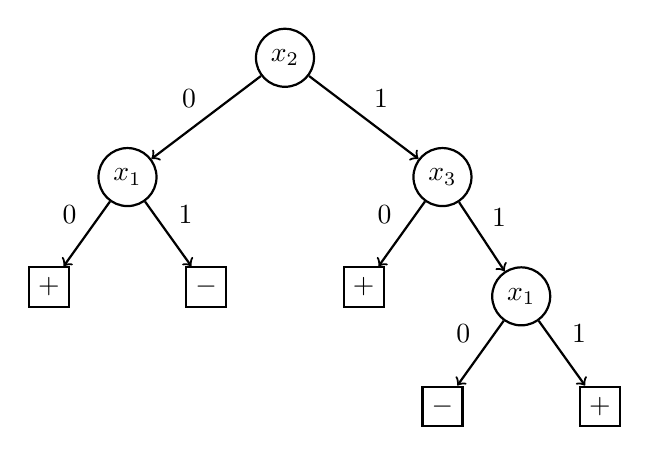
\begin{tikzpicture}[
    auto, thick,
    node/.style={draw, circle, thick, text centered, 
    minimum height=0.50cm, minimum width=0.50cm},
    star/.style={draw, diamond, thick, text centered, 
    minimum height=0.50cm, minimum width=0.50cm},
    block/.style={draw, thick, text centered, 
    minimum height=0.50cm, minimum width=0.50cm},
    title/.style={draw=none, circle, thick, text centered, 
    minimum height=0.50cm, minimum width=0.50cm},
    every loop/.style={}
    ]
    \node[node]   (x2)                                        {$x_2$};
    \node[node]   (x1)  [below=0.75 of x2, xshift=-2.00cm]    {$x_1$};
    \node[node]   (x3)  [below=0.75 of x2, xshift= 2.00cm]    {$x_3$};
    \node[node]   (x4)  [below=0.75 of x3, xshift= 1.00cm]    {$x_1$};
    
    \node[block]  (y1)  [below=0.75 of x1, xshift=-1.00cm]    {$+$};
    \node[block]  (y2)  [below=0.75 of x1, xshift= 1.00cm]    {$-$};
    \node[block]  (y3)  [below=0.75 of x3, xshift=-1.00cm]    {$+$};
    \node[block]  (y4)  [below=0.75 of x4, xshift=-1.00cm]    {$-$};
    \node[block]  (y5)  [below=0.75 of x4, xshift= 1.00cm]    {$+$};
    
    \path[->]
    (x2)  edge  node[above left]  {$0$}  (x1)
    (x2)  edge  node[above right] {$1$}  (x3)
    (x1)  edge  node[above left]  {$0$}  (y1)
    (x1)  edge  node[above right] {$1$}  (y2)
    (x3)  edge  node[above left]  {$0$}  (y3)
    (x3)  edge  node[above right] {$1$}  (x4)
    (x4)  edge  node[above left]  {$0$}  (y4)
    (x4)  edge  node[above right] {$1$}  (y5)
    ;
  \end{tikzpicture}

  Fórmula booleana equivalente: $\overline{x_1}\overline{x_2}\lor x_2\overline{x_1}\lor x_1x_2x_3$.

  {
    \delimitershortfall=-1pt                        % bigger wrapping brackets
    $\mathcal{L}$: 
    $\l(x_2
            \l(x_1
                  \l(+\r)
                  \l(-\r)
            \r)
            \l(x_3
                  \l(+\r)
                  \l(x_1
                      \l(-\r)
                      \l(+\r)
                  \r)
            \r)
      \r)$
  }

  Alfabeto: $\l\{1,\ \ldots,\ d\r\}\cup\l\{\text{'('},\ \text{')'},\ \text{'+'},\ \text{'-'}\r\}$, $\l\lceil\lg\l(d+4\r)\r\rceil$ bits por símbolo.
\end{exemplo}

\begin{exercicio}
  Seja $f(k)$ o número de símbolos que precisamos para representar uma árvore de decisão com $k$ nós externos em $\mathcal{L}$. Prove que
  \[
    f(k) = 3\cdot\l(2\cdot k-1\r),\ k\geq 1
  \]

  Representação de uma árvore de decisão com $k$ nós externos:
  \[
    3\cdot\l(2\cdot k-1\r)\cdot\l\lceil\lg\l(d+4\r)\r\rceil = \mathcal{O}\l(k\cdot\log d\r) \text{bits}
  \]
\end{exercicio}
\begin{resolucao}
  Os $k$ nós externos contribuem com $3$ símbolos cada: '(+)' ou '(-)'.

  Os $k-1$ nós internos contribuem com $3$ símbolos cada: '(x' e ')'

  Resultado: $3\cdot k + 3\cdot\l(k-1\r) = 3\cdot\l(2\cdot k-1\r)$.

  O fator $\cdot\l\lceil\lg\l(d+4\r)\r\rceil$ é pela quantidade mínima de bits para representar o alfabeto.
\end{resolucao}

Dado $\mathrm{S}\subseteq\l\{0,\ 1\r\}^d$, como obtemos uma Árvore de Decisão $T$ com $\mathrm{err}_\mathrm{S}\l(T\r)=0$?

\begin{exercicio}
  Fácil obter uma $T$ com $\leq2\cdot\l|\mathrm{S}\r|$ nós externos.
\end{exercicio}
\begin{resolucao}
  Uma árvore balanceada com $2^d=\l|\mathrm{S}\r|$ nós externos é capaz de estilhaçar $\mathrm{S}\subseteq\l\{0,\ 1\r\}^d$
\end{resolucao}

Assim
\[
  \mathrm{size}\l(T\r) = \mathcal{O}\l(\l|\mathrm{S}\r|\log d\r).
\]

Se conseguimos $T$ com (pelo Teo 4 (ref:label?))
\[
  \mathrm{size}\l(T\r) \leq \frac{\eps}{2\cdot\log 2} \l|\mathrm{S}\r|
\]

e $\l|\mathrm{S}\r|\geq\frac{2}{\eps}\cdot\log\nicefrac{1}{\delta}$, então com prob. $\geq 1-\delta$,
\begin{align}
  \mathrm{err}_\mathcal{D}\l(T\r) &\leq \frac{\mathrm{size}\l(T\r)\cdot\log2 + \log\nicefrac{1}{\delta}}{\l|\mathrm{S}\r|}  \\
                                  &\leq \frac{\eps}{2} + \frac{\eps}{2} = \eps
\end{align}

Podemos deduzir algo análogo para o Teo. 5 (ref:label?).

\begin{fato}
  Obter uma menor $T$ tal que $\mathrm{err}_\mathrm{S}\l(T\r)=0$ é NP-difícil.
\end{fato}
%endregion

%region Iterative dichotomizer
\clearpage
\subsection{Heurística ID3}

\paragraph{\nopunct}[\textit{Sugestão: <\href{https://en.wikipedia.org/wiki/Mutual\_information}{https://en.wikipedia.org/wiki/Mutual\_information}>}]

Considere a partição $\mathrm{S}=\mathrm{S}^+\cup\mathrm{S}^-$ de instâncias positivas e negativas.

Seja também a indicação $\mathrm{S}_{x_i=0}\defeq\l\{s\in \mathrm{S}\colon\ x_i=0\r\}$

\begin{definicao}
  \normalfont
  \textbf{Entropia binária}
  \[
    \mathrm{H}\l(p\r) = \mathrm{H}_2\l(p\r) \defeq p\cdot\lg\nicefrac{1}{p} + q\cdot\lg\nicefrac{1}{q}
  \]

  onde $p+q=1$ e $0\leq 0\leq1$.

  Convenção: $0\cdot\log\nicefrac{1}{0}=0\cdot\log0=0$
\end{definicao}

\[
  \mathrm{H}\l(\mathrm{S}\r) = \mathrm{H}\l(\nicefrac{\l|\mathrm{S}^+\r|}{\l|\mathrm{S}\r|}\r)
\]

\[
  \mathrm{H}\l(\mathrm{S}\given x_i\r) = \frac{\mathrm{S}_{x_i=0}}{\mathrm{S}}\cdot\mathrm{H}\l(\mathrm{S}_{x_i=0}\r) + \frac{\mathrm{S}_{x_i=1}}{\mathrm{S}}\cdot\mathrm{H}\l(\mathrm{S}_{x_i=1}\r)
\]

\begin{definicao}
  \normalfont
  Heurística: escolhemos $x_i$ para minimizar o ganho de informação.

  \textbf{Information Gain:}
  \[
    \mathrm{IG}\l(i\r) \defeq \mathrm{H}\l(S\r) - \mathrm{H}\l(\mathrm{S}\given x_i\r).
  \]

  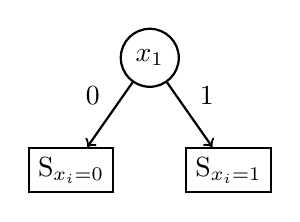
\begin{tikzpicture}[
    auto, thick,
    node/.style={draw, circle, thick, text centered, 
    minimum height=0.50cm, minimum width=0.50cm},
    star/.style={draw, diamond, thick, text centered, 
    minimum height=0.50cm, minimum width=0.50cm},
    block/.style={draw, thick, text centered, 
    minimum height=0.50cm, minimum width=0.50cm},
    title/.style={draw=none, circle, thick, text centered, 
    minimum height=0.50cm, minimum width=0.50cm},
    every loop/.style={}
    ]
    \node[node]   (x1)                                        {$x_1$};
    
    \node[block]  (y1)  [below=0.75 of x1, xshift=-1.00cm]    {$\mathrm{S}_{x_i=0}$};
    \node[block]  (y2)  [below=0.75 of x1, xshift= 1.00cm]    {$\mathrm{S}_{x_i=1}$};
    
    \path[->]
      (x1)  edge  node[above left]  {$0$}  (y1)
      (x1)  edge  node[above right] {$1$}  (y2)
    ;
  \end{tikzpicture}
\end{definicao}
%endregion

}
